\documentclass{beamer}

\usepackage[utf8]{inputenc}
\usepackage[russian]{babel}
\usepackage{hyperref}
\usepackage{graphicx}
\usepackage{listings}

\usetheme{Warsaw}
\usecolortheme{lily}
\useoutertheme[subsection=false]{smoothbars}
\useinnertheme{circles}
\setbeamertemplate{footline}[page number]{}
\setbeamertemplate{navigation symbols}{}

\title{Архитектура ЭВМ}
\subtitle{Лекция 1. Как работает компьютер?}
\author{к.ф.-м.н. Филонов Павел Владимирович \\ filonovpv@gmail.com}
\date{2 сентября 2013 г.}

\institute[МГТУ ГА] 
{
    Московский Государственный Технический Университет \\
    Гражданской Авиации
}
\begin{document}
    \frame{\titlepage}
    \section{Введение}
    \subsection{}
    \begin{frame}{О чём курс?}
        \begin{itemize}
            \item Формально:\\
            {\bf Архитекутра ЭВМ} --- концептуальная структура ВМ, определяющая проведение обработки информации и включающая методы преобразования информации в данные и принципы взаимодействия технических средств и программного обеспечения\footnote{ГОСТ 15971-90 Системы обработки информации. Термины и определения.}
            \bigskip

        \item Попроще:
        \begin{itemize}
            \item Как работает компьютер?
            \item Что такое x86, x86\_64 и пр. ?
            \item Что такое ассемблер и зачем он нужен?
            \item Во что превращается код на Pascal, C и пр.?
        \end{itemize}
        \end{itemize}
    \end{frame}
    \begin{frame}{Где это практически нужно?}
        \begin{itemize}
            \item Дизассемблирование (crack)
            \item Внедрение кода (exploit)
            \item Создание компиляторов
            \item Написание низкоуровневой части ОС
            \item "Искусство программирования" Д.~Кнута
            \item Оптимизация времени выполнения
        \end{itemize}
    \end{frame}
    \begin{frame}[fragile]
    \frametitle{{Дизассемблирование (crack)}}
        Что делает эта программа?
\begin{verbatim}
8048464:   55            push   %ebp
8048465:   89 e5         mov    %esp,%ebp
8048467:   83 e4 f0      and    $0xfffffff0,%esp
804846a:   83 ec 20      sub    $0x20,%esp
804846d:   c7 44 24 14   movl   $0x0,0x14(%esp)
8048474:   00 
8048475:   c7 44 24 18   movl   $0x0,0x18(%esp)
804847c:   00 
804847d:   eb 3c         jmp    80484bb <main+0x57>
804847f:   e8 1c ff ff   call   80483a0 <__ctype_b_loc@plt>
8048484:   8b 00         mov    (%eax),%eax
8048486:   8b 54 24 1c   mov    0x1c(%esp),%edx
804848a:   01 d2         add    %edx,%edx
804848c:   01 d0         add    %edx,%eax
804848e:   0f b7 00      movzwl (%eax),%eax
\end{verbatim}
\end{frame}
    \begin{frame}[fragile]
    \frametitle{Внедрение кода (exploit)}
    \begin{block}{Пример Шелл-кода}
    \begin{verbatim}
http://www.enderunix.org/documents/eng/bof-eng.txt 
char sc[]=              /* 24 bytes                 */
    "\x31\xc0"             /* xorl    %eax,%eax     */
    "\x50"                 /* pushl   %eax          */
    "\x68""//sh"           /* pushl   $0x68732f2f   */
    "\x68""/bin"           /* pushl   $0x6e69622f   */
    "\x89\xe3"             /* movl    %esp,%ebx     */
    "\x50"                 /* pushl   %eax          */
    "\x53"                 /* pushl   %ebx          */
    "\x89\xe1"             /* movl    %esp,%ecx     */
    "\x99"                 /* cdql                  */
    "\xb0\x0b"             /* movb    $0x0b,%al     */
    "\xcd\x80"             /* int     $0x80         */
;
    \end{verbatim}
    \end{block}
\end{frame}
    \begin{frame}[fragile]
    \frametitle{Создание компиляторов}
    \begin{columns}
    \column{0.8\linewidth}
    Хотите написать свой язык программирования?
    \begin{block}{Kaleidoscope (http://llvm.org/docs/tutorial/)}
        \begin{verbatim}
def foo(a b) a*a + 2*a*b + b*b;   
        \end{verbatim}
    \end{block}
    \column{0.2\linewidth}
    
\includegraphics[width=\linewidth]{fig/llvm-logo.jpeg}
    \end{columns}
    \begin{block}{Пример трансляции: LLVM --- Low Level Virtual Machine}
\begin{verbatim}
define double @foo(double %a, double %b) {
entry:
  %multmp = fmul double %a, %a
  %multmp1 = fmul double 2.000000e+00, %a
  %multmp2 = fmul double %multmp1, %b
  %addtmp = fadd double %multmp, %multmp2
  %multmp3 = fmul double %b, %b
  %addtmp4 = fadd double %addtmp, %multmp3
  ret double %addtmp4
}
\end{verbatim}
    \end{block}
\end{frame}
    \begin{frame}[fragile]
    \frametitle{Написание низкоуровневой части ОС}
\begin{columns}
\column{0.5\linewidth}
    \begin{block}{Linux 0.01 Bootloader}\small
\begin{verbatim}
entry start
start:
    mov ax,#BOOTSEG
    mov ds,ax
    mov ax,#INITSEG
    mov es,ax
    mov cx,#256
    sub si,si
    sub di,di
    rep
    movw
    jmpi    go,INITSEG
go: mov ax,cs
    mov ds,ax
    mov es,ax
    mov ss,ax
    mov sp,#0x400       
\end{verbatim}    
    \end{block}
    \column{0.5\linewidth}
    
\includegraphics[width=\linewidth]{fig/linux-logo.jpg}
    \end{columns}
\end{frame}
    \begin{frame}{<<Искусство программирования>> Д.~Кнута}
        \begin{columns}
            \column{0.8\linewidth}
            Во всех томах <<Искусства программирования>> все примеры
            приведены на машинном языке MIX
            \column{0.2\linewidth}
            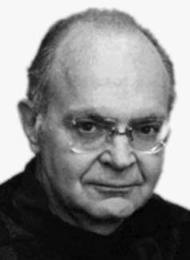
\includegraphics[width=\linewidth]{fig/Knuth.jpeg}
        \end{columns}
        \begin{figure}
            \begin{minipage}[h]{0.3\linewidth}
                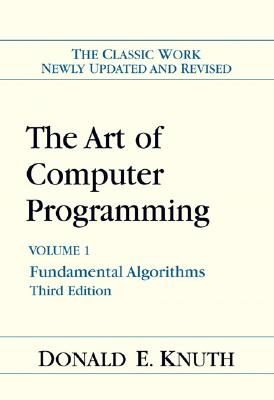
\includegraphics[width=0.8\linewidth]{fig/TAoP1.jpg}
            \end{minipage}
            \begin{minipage}[h]{0.33\linewidth}
                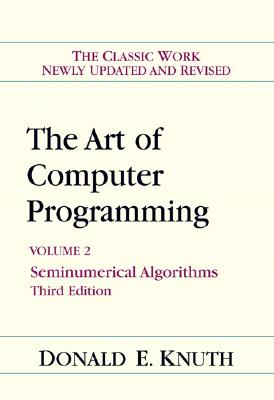
\includegraphics[width=0.8\linewidth]{fig/TAoP2.jpg}
            \end{minipage}
            \begin{minipage}[h]{0.33\linewidth}
                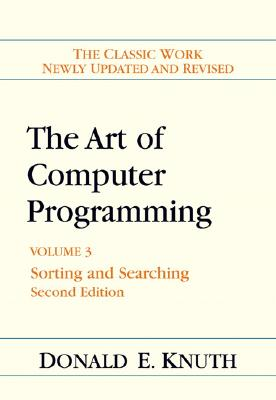
\includegraphics[width=0.8\linewidth]{fig/TAoP3.jpg}
            \end{minipage}
        \end{figure}    
    \end{frame}
    \begin{frame}[fragile]
        \frametitle{Оптимизация времени выполнения}
        \begin{block}{Копирование матриц (а)}
        \begin{verbatim}
for i := 1 to N do
    for j := 1 to N do
        dst[i,j] := src[i,j];
        \end{verbatim}   
        \end{block}
        \begin{block}{Копирование матриц (б)}
        \begin{verbatim}
for j := 1 to N do
    for i := 1 to N do
        dst[i,j] := src[i,j];
        \end{verbatim}   
        \end{block}
        Какой из вариантов быстрее? \\
        \pause
        \color{red}{Вариант (б) работает быстрее в 6 раз}
\end{frame}
    \begin{frame}{Что нас ждёт?}
        \begin{itemize}
            \item Лекции - 20 часов (10 лекций)
            \item Семинары - 11 часов (5 семинаров)
            \item Лабораторные работы - 20 часов (5 работ)
            \item Домашние задания - 3 ДЗ (ejudge)
            \item Зачёт
        \end{itemize}
    \end{frame}
    \begin{frame}{Что на поможет?}
        \begin{itemize}
            \item {\bf Основная литература}
            \begin{itemize}
                \item А.В.~Столяров. Программирование на языке ассемблера NASM для ОС UNIX. 2-е изд. --- \url{http://stolayrov.info/books/asm_unix}
            \end{itemize}
            \item {\bf Дополнительная литература}
            \begin{itemize}
                \item Ч.~Петцольд. Код. Тайный язык информатики
                \item Ю.~Магда. Ассемблер для процессоров Intel Pentium
                \item Э.~Таненбаум. Архитектура компьютера. 5-е изд.
            \end{itemize}
            \item {\bf Internet--ресурсы}
            \begin{itemize}
                \item Сайт дисциплины --- \url{http://cleric.su/pm/asm}
                \item Лекция по Архитектуре ЭВМ с Yandex КИТ --- \url{http://events.yandex.ru/events/kit/2/talks/591/}
                \item Видеокурс Архитетура ЭВМ на Intuit.ru--- \url{http://www.intuit.ru/studies/courses/535/391/info}
                \item Intel® 64 and IA-32 Architectures Software Developer Manuals --- \url{http://www.intel.com/content/www/us/en/processors/architectures-software-developer-manuals.html}
            \end{itemize}
        \end{itemize}
    \end{frame}
    \begin{frame}{Вопросы}
        \begin{block}{Как меня зовут?}
            \begin{enumerate}
                \item<2-> Павлов Владимир Филонович
                \item<3-> Филонов Владимир Павлович
                \item<4-> Владимиров Филон Павлович
                \item<5-> \alt<6>{\color{green}Филонов Павел Владимирович}{Филонов Павел Владимирович}
            \end{enumerate}
        \end{block}
        \pause
    \end{frame}
    \begin{frame}{Вопросы}
        \begin{block}{Как называется предмет?}
            \begin{enumerate}
                \item<2-> Архитектура инженерных сооружений
                \item<3-> Архитектура 
                \item<4-> \alt<6>{\color{green}Архитектура ЭВМ}{Архитектура ЭВМ}
                \item<5-> Архитектура ЭВМ и язык ассемблера
            \end{enumerate}
        \end{block}
        \pause
    \end{frame}
    \begin{frame}{Вопросы}
    \centerline{\Huge Ваши вопросы?}
    \end{frame}

    \section{Архитектура фон Неймана}
    \subsection{}
    \begin{frame}{Архитектура фон Неймана}
        \transdissolve
        \begin{figure}
            \centering
            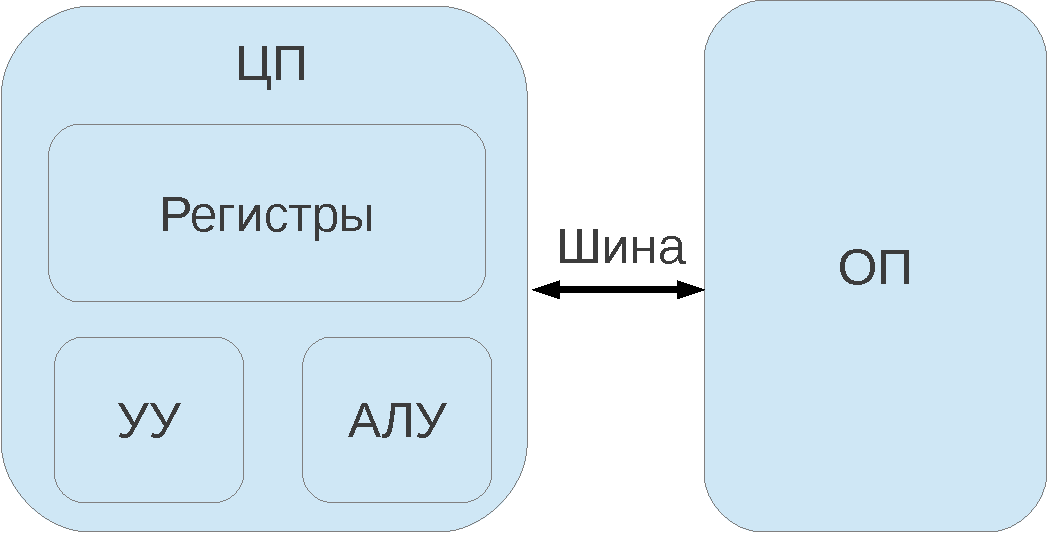
\includegraphics[width=0.8\linewidth]{fig/arch.pdf} 
        \end{figure}
        {\bf ЦП} --- центральный процессор (CPU --- central processing unit) \\
        {\bf ОП} --- оперативная память (RAM --- random access memory) \\
        {\bf Регистр} --- ячейка памяти (register)\\
        {\bf УУ} --- устройство управления (CU --- control unit)\\
        {\bf АЛУ} --- арифметико-логическое устройство (ALU --- arithmetic logic unit)\\
    \end{frame}
    \begin{frame}{Принципы фон Неймана}
        \begin{enumerate}
            \item Двоичное кодирование информации
            \item Однородность памяти --- неразличимость команд и данных
            \item Адресуемость памяти --- память состоит из пронумерованных ячеек
            \item Программное управление --- последовательное выполнение команд
        \end{enumerate}
        \begin{columns}
        \column{0.39\linewidth}
            EDVAC --- Electronic Discrete Variable Automatic Computer, установленный в здании Лаборатории баллистических исследований (1949 г.)
        \column{0.59\linewidth}
            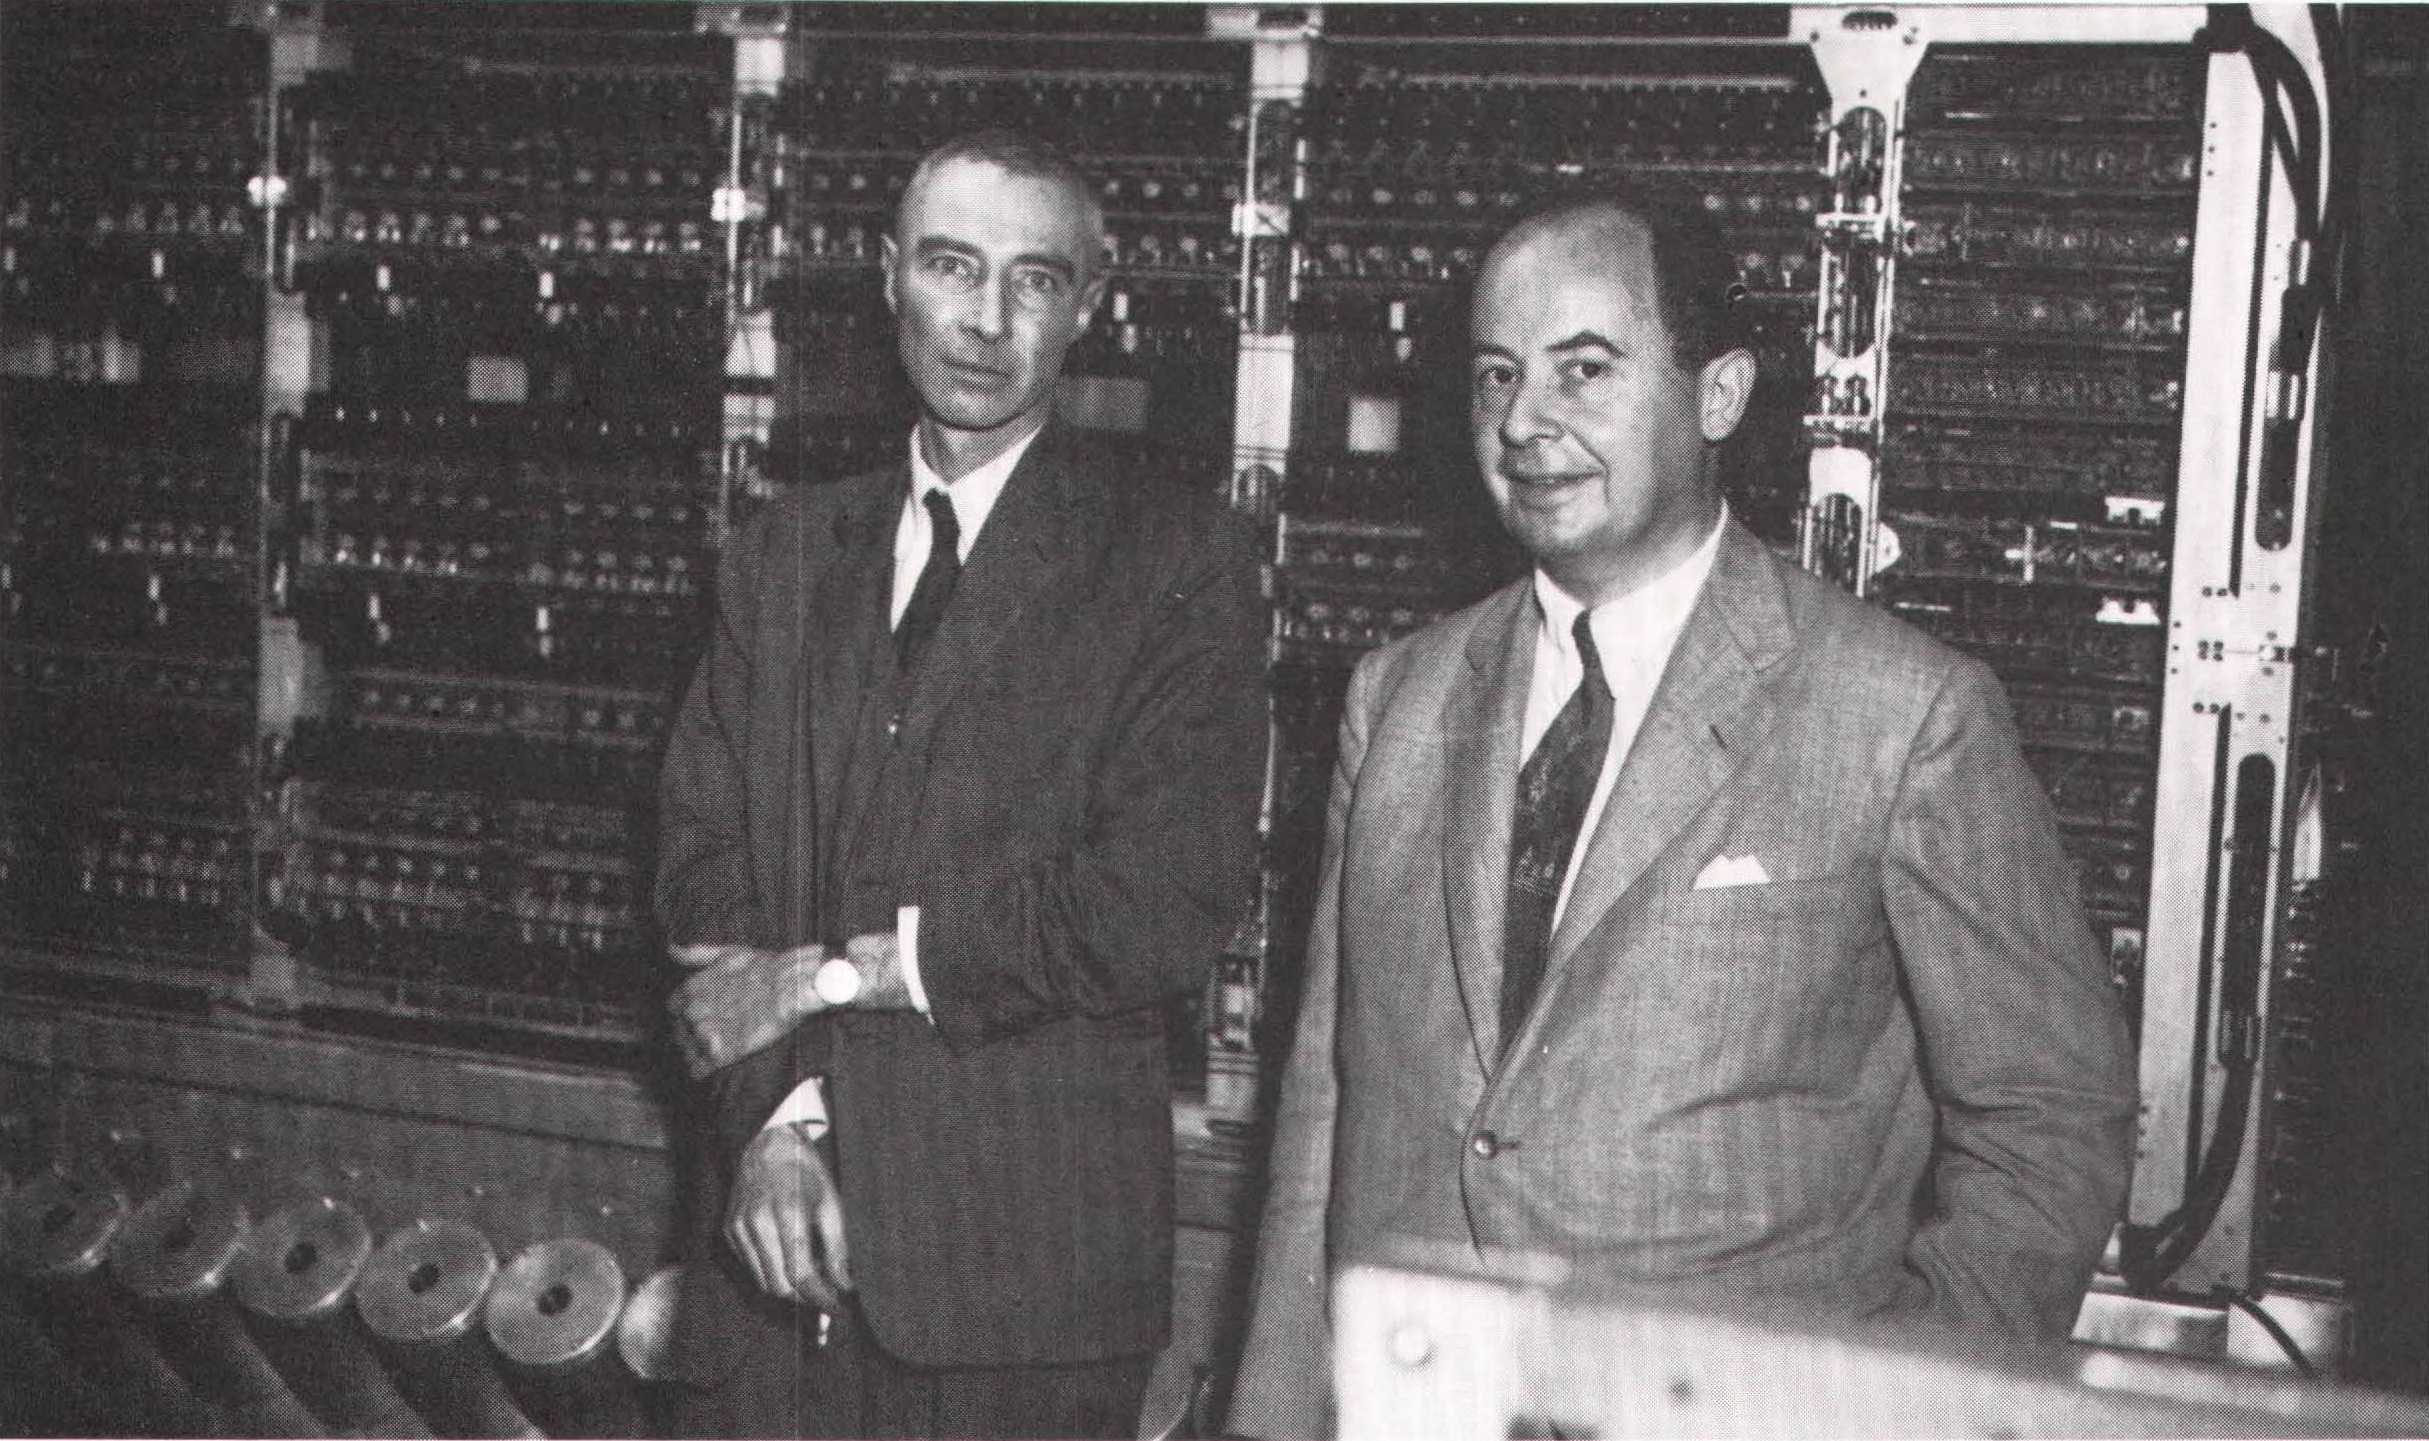
\includegraphics[width=1.0\linewidth]{fig/EDVAC.jpg}
        \end{columns}
    \end{frame}
    \begin{frame}{Упрощенный цикл работы}

        {\bf Счётчик команд} --- специальный регистр, хранящий адрес следующей исполняемой команды \\
        {\bf Машинная команда } --- элементарная операция, которая может быть выполнена ЦП
        \bigskip
        \begin{enumerate}
            \item Положить в {\it счётчик команд} (СК) начальный адрес 
            \item Извлечь команду из памяти по адресу, который содержится в СК
            \item Увеличить СК на размер команды
            \item Выполнить команды
            \item Перейти на шаг 2
        \end{enumerate}
    \end{frame}
    \begin{frame}{Разминка}
        \begin{block}{Что такое регистр?}
            \begin{enumerate}
            \item Специальная ячейка оперативной памяти
            \item \alt<2>{{\color{green}Ячейка памяти в центральном процессоре}}{Ячейка памяти в центральном процессоре} 
            \item Устройство для арифметических действий
            \item Периферийное устройство
            \end{enumerate}
        \end{block}
    \end{frame}
    \begin{frame}{Разминка}
        \begin{block}{Принципы фон Неймана составляют:}
            \begin{enumerate}
            \item \alt<2>{{\color{red}Разделение каналов команд и данных}}{Разделение каналов команд и данных}
            \item \alt<2>{{\color{green}Однородность памяти}}{Однородность памяти}
            \item \alt<2>{{\color{red}Десятичное кодирование}}{Десятичное кодирование}
            \item \alt<2>{{\color{green}Двоичное кодирование}}{Двоичное кодирование}
            \item \alt<2>{{\color{green}Программное управление}}{Программное управление}
            \item \alt<2>{{\color{green}Адресуемость памяти}}{Адресуемость памяти}
            \item \alt<2>{{\color{red}Разделение команд и данных}}{Разделение команд и данных}
            \end{enumerate}
        \end{block}
    \end{frame}

    \section{KiD}
    \subsection{}
    \begin{frame}{Пример: KiD}
        Давайте придумаем свой компьютер на основе архитектуры фон Неймана
        \begin{figure}
            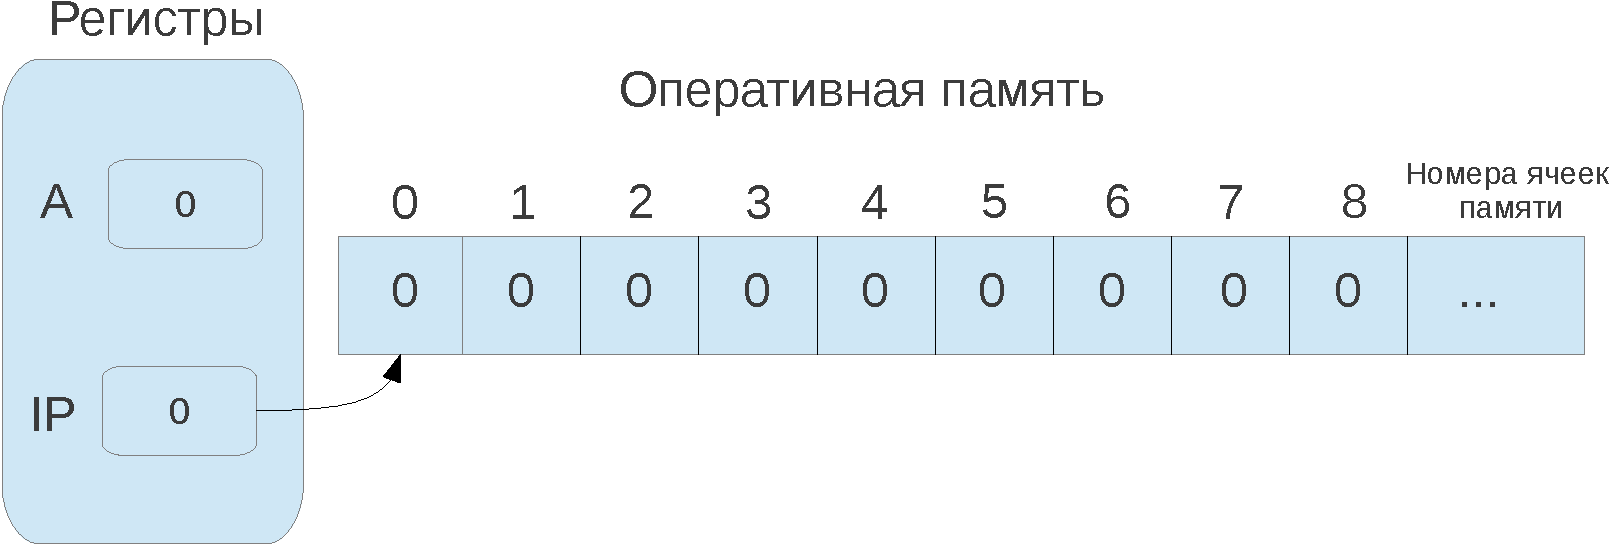
\includegraphics[width=1.0\linewidth]{fig/KiD.pdf}
        \end{figure}
        {\bf A } --- регистр общего назначения \\
        {\bf IP} (Instruction Pointer) --- счётчик команд \\
        {\it Оперативная память} состоит из {\it ячеек}. Каждая ячейка имеет номер начиная с нуля ({\it адрес ячейки}) и значение ({\it содержимое ячейки})
    \end{frame}
    \begin{frame}[fragile]
        \frametitle{Пример: KiD}
        \begin{tabular}{|c|c|c|l|p{0.4\linewidth}|}
            \hline \bf Код & \bf Формат & \bf Размер & \bf Мнемоника & \bf Описание \\
            \hline 10 & 10 X & 2 & A := X & \small Загрузить в A значение X \\
            \hline 20 & 20 X & 2 & A := A + X & \smallПрибавить к A значение X \\
            \hline 21 & 21 X & 2 & A := A - X & \smallВычесть из A значение X \\
            \hline 77 & 77 & 1 & HLT & \small Остановить работу \\
            \hline
        \end{tabular}
        \begin{block}{Напишем программу для вычисления выражения 51-43+32:}
        \begin{verbatim}
Мнемонические    Машинные
 обозначения       Коды
A := 51            10 51
A := A - 43        21 43
A := A + 32        20 32
HLT                77
        \end{verbatim}
        \end{block}
\end{frame}
    \begin{frame}{Пример: KiD}
        \begin{figure}[t]
            \only<1>{
                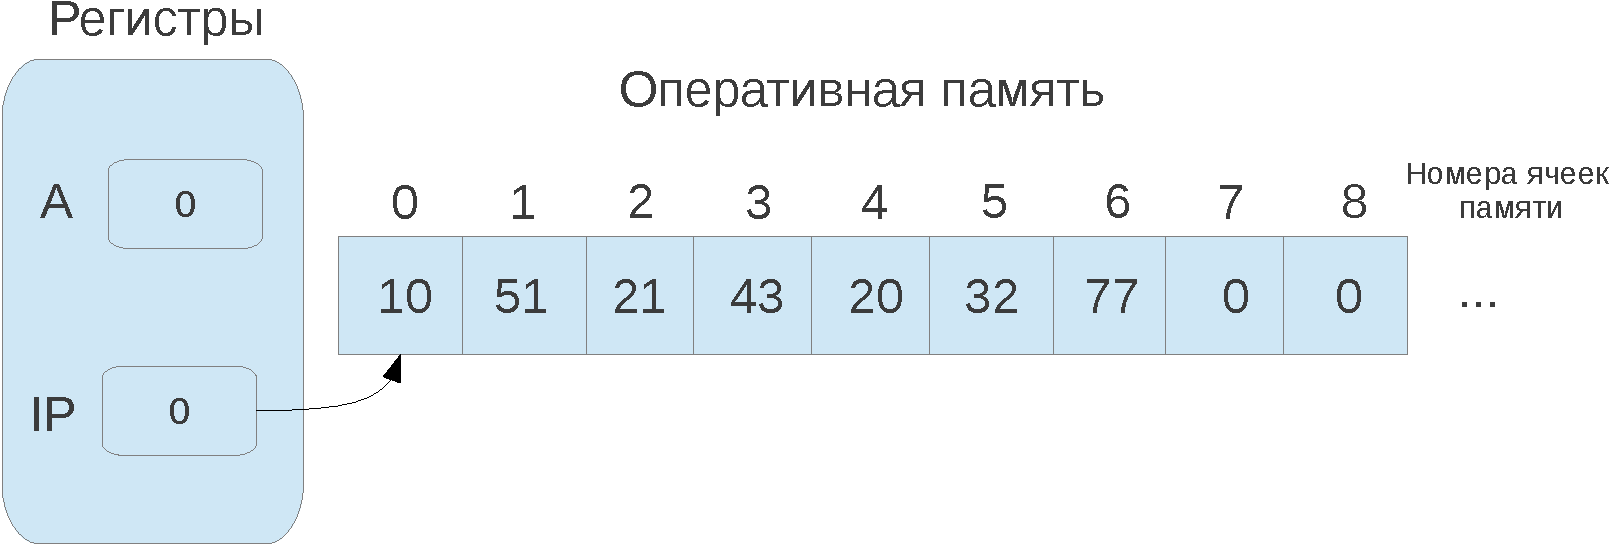
\includegraphics[width=1.0\linewidth]{fig/KiD1.pdf}
                \begin{block}{Подготовка}
                    \begin{enumerate}
                        \item Загрузим нашу программу в ОП начиная с нулевого адреса
                        \item Обнулим значение IP
                    \end{enumerate}
                \end{block}
            }
            \only<2>{
                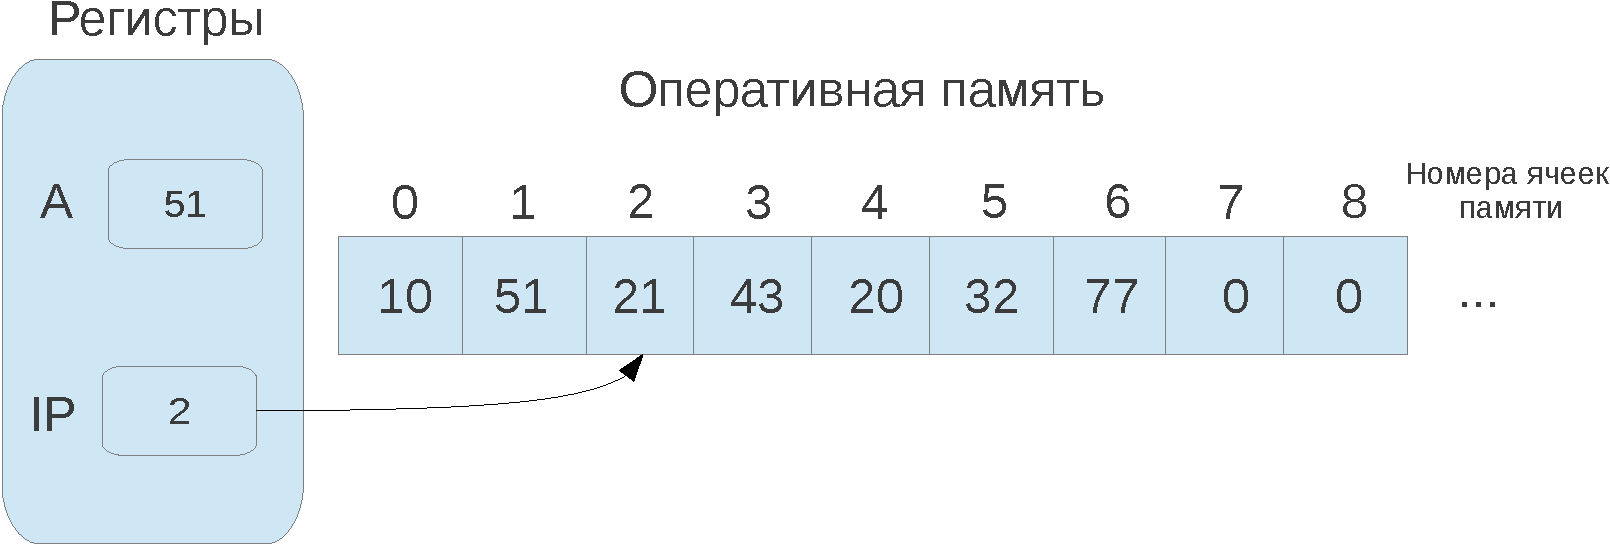
\includegraphics[width=1.0\linewidth]{fig/KiD2.pdf}
                \begin{block}{Итерация цикла}
                    \begin{enumerate}
                        \item Считаем команду Загрузить (10) и её операнды
                        \item Увеличим IP на 2
                        \item Выполним A := 51
                    \end{enumerate}
                \end{block}
            }
            \only<3>{
                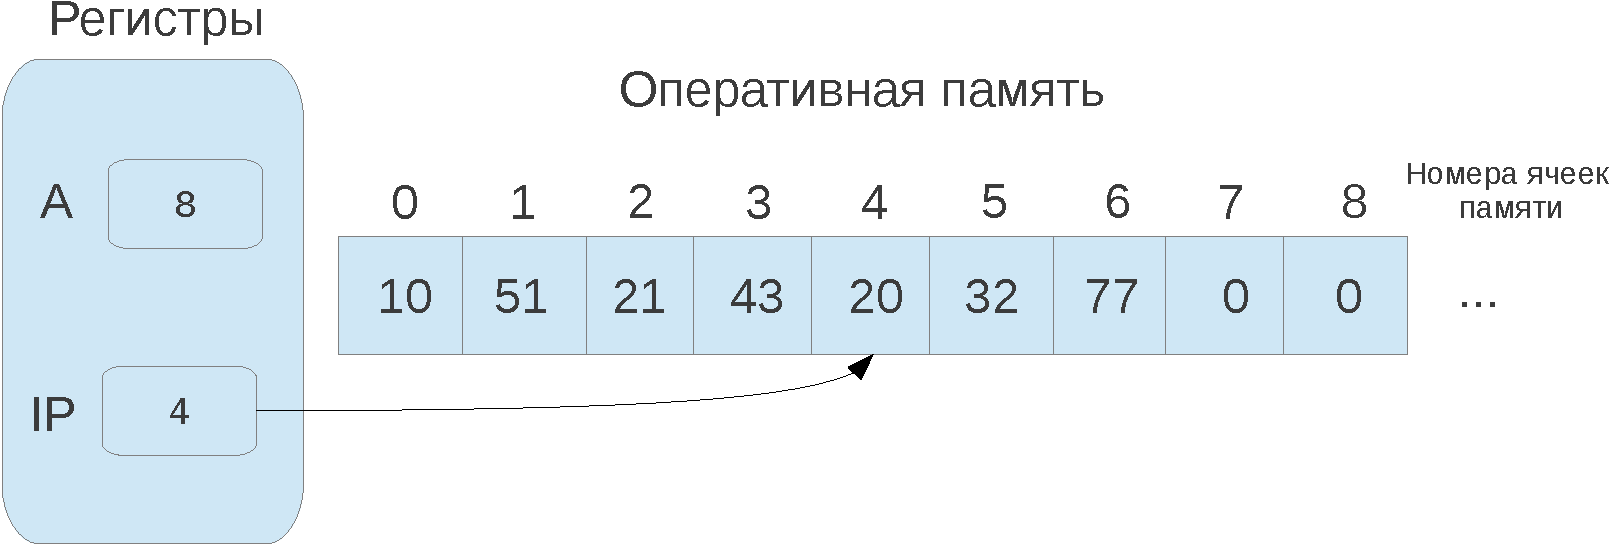
\includegraphics[width=1.0\linewidth]{fig/KiD3.pdf}
                \begin{block}{Итерация цикла}
                    \begin{enumerate}
                        \item Считаем команду Вычесть (21) и её операнды
                        \item Увеличим IP на 2
                        \item Выполним A := A - 43
                    \end{enumerate}
                \end{block}
            }
            \only<4>{
                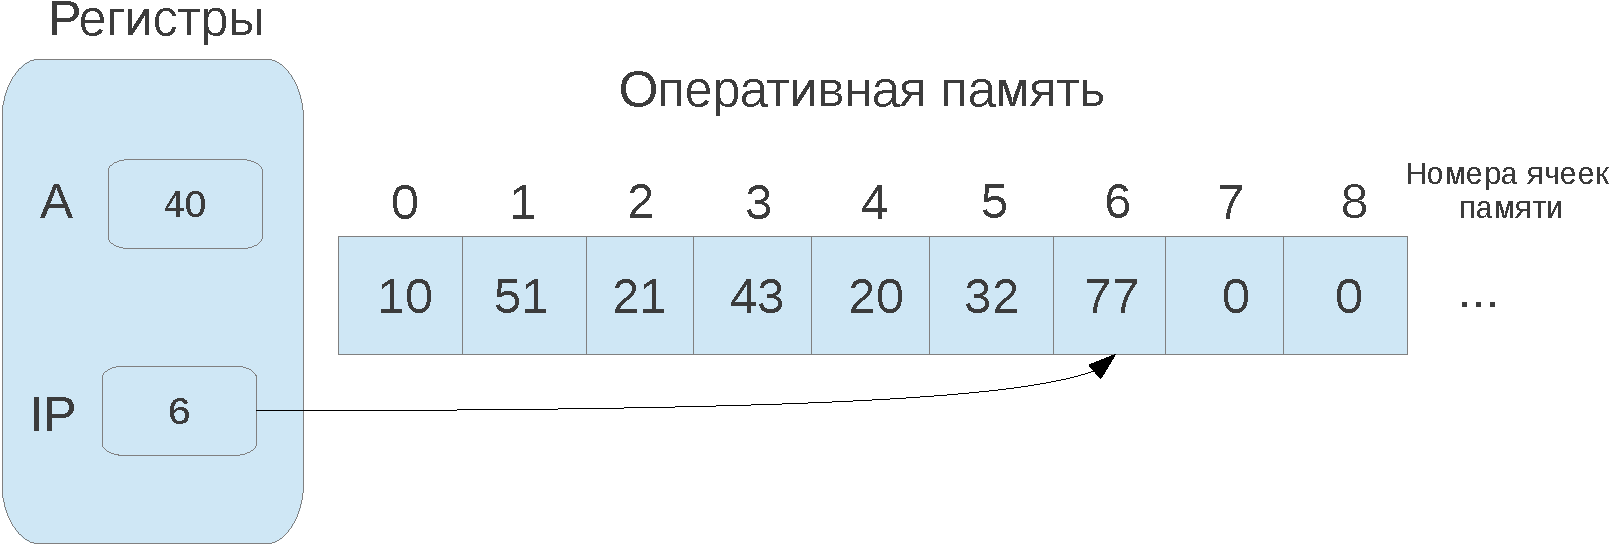
\includegraphics[width=1.0\linewidth]{fig/KiD4.pdf}
                \begin{block}{Итерация цикла}
                    \begin{enumerate}
                        \item Считаем команду Прибавить (20) и её операнды
                        \item Увеличим IP на 2
                        \item Выполним A := A + 32
                    \end{enumerate}
                \end{block}
            }
            \only<5>{
                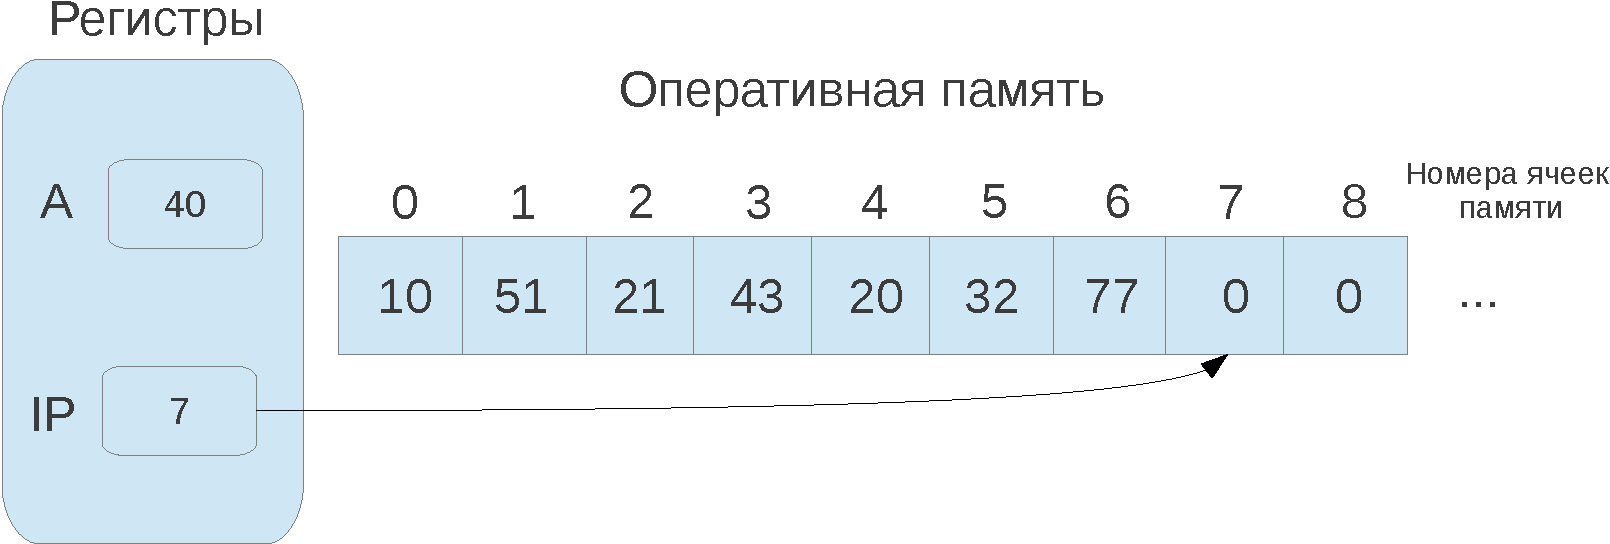
\includegraphics[width=1.0\linewidth]{fig/KiD5.pdf}
                \begin{block}{Итерация цикла}
                    \begin{enumerate}
                        \item Считаем команду Остановить (77)
                        \item Увеличим IP на 1
                        \item Остановка
                    \end{enumerate}
                \end{block}
            }            
        \end{figure}
    \end{frame}
    \begin{frame}{Разминка}
        \begin{block}{Что делает команда 20 20}
            \begin{enumerate}
                \item Ничего
                \item Вычисляет факториал 20
                \item Загружает в регистр A значение 20
                \item \alt<2->{{\color{green}Прибавляет к регистру A число 20}}{Прибавляет к регистру A число 20}
                \end{enumerate}
        \end{block}
        \pause
        \begin{block}{Чему будет равно значение регистра A после выполнения следующей программы: \\
         10 11 20 3 20 20 21 20 20 5 77}
            Ответ: \pause 19
        \end{block}
    \end{frame}

    \section{Заключение}
    \subsection{}
    \begin{frame}
        \begin{block}{Что мы узнали?}
            \begin{enumerate}
                \item Как называется предмет. Как зовут преподавателя. Как называется книжка.
                \item Зачем это может пригодится.
                \item Кто такой фон Неймана.
                \item Какие принципы лежат в основе архитектуры {\bf всех} современных ЭВМ.
                \item Что такое ЦП, ОП, УУ, АЛУ, регистр, СК, машинный код.
                \item Научились выполнять работу процессора (выполнять машинный код)
            \end{enumerate}
        \end{block}
    \end{frame}
\end{document}